\chapter{Bayes'sches Netz}
Dieses Kapitel beschäftigt sich eingangs mit den Grundlagen von Bayes'schen Netzen. Ein Beispiel soll den Sachverhalt greifbar erklären.

\section{Eigenschaften von Bayes'schen Netzen}
In der Vorlesung \cite{Strand17} wurde thematisiert, dass ein Roboter zur Lokalisierung über mehrere Sensorsysteme verfügt. Hintergrund ist der, dass die verschiedenen Systeme alle fehlerbehaftet sind. Jedes in einer anderen Hinsicht. So kann es beispielsweise bei der Messung der Raddrehung durch Schlupf zu Messfehlern kommen.

Sei nun \textit{n} die Anzahl der Sensorsysteme und \textit{m} der Wertebereich der möglichen Trefferwahrscheinlichkeiten der Sensorsysteme, dann beträgt der Aufwand der Auswertung des stochastischen Ausdrucks \[ m^n\] Somit wächst der Aufwand von der Auswertung des Ausdrucks exponentiell. Dieser Aufwand kann in der Praxis glücklicherweise jedoch meist minimiert werden. Oft kann man auf Variablen verzichten, ohne einen Informationsverlust herbeizurufen. Hier kommen Bayes'sche Netze ins Spiel. Sie verwenden das das Wissen über unabhängige Variablen. 
\subsection{Unabhängige Variablen}
Sind Zufallsvariablen paarweise unabhängig, so gilt: \[ P(X_1, ..., X_n) = P(X_1) * P(X_2) * ... * P(X_n)\] 
Und: \[ P(A\vert B) = \frac{P(A,B)}{P(B)} = \frac{P(A) * P(B)}{P(B)}  = P(A) \] da sich \textit{P(B)} rauskürtzt. Man spricht davon, dass sich \textit{P(A$\vert$ B)} auf die \textit{A-pri"-ori-Wahr"-schein"-lich"-keit} reduziert. Die A-pri"-ori-Wahr"-schein"-lich"-keit beschreibt die Wahrscheinlichkeit, die man durch Vorwissen annehmen kann, in diesem Fall die Unabhängigkeit. Nun kann es jedoch auch sein, dass nicht für alle Variablen paarweise Unabhängigkeit gilt. Es folgt nun ein Beispiel nach \cite{Perl88}. Es soll aufzeigen, wie man mit Bayes'schen Netzen auf Sachverhalte schließen kann und dabei auch Abhängigkeiten von Variablen nutzt. 

\section{Alarmanlagen-/Erdbebenbeisiel}
Bob ist alleinstehend und berufstätige und möchte sein Haus vor Einbrechern schützen. Er bringt in seinem Haus eine Alarmanlage an. Sie soll im Falle eines Einbruches (\textit{Ein}) alarmieren. Da er im Büro ist, kann er den Alarm nicht hören. Glücklicherweise hat er die netten Nachbarn John (\textit{J}) und Mary (\textit{M}). Sie wohnen im linken beziehungsweise rechten Nachbarhaus. John hat nun schon einige Jahre Erfahrung mit seiner Alarmanlage (\textit{Al}) und dem Anrufverhalten seiner Nachbarn und weiß: 
\[ P(J\vert Al) = 0,9\] 
\[ P(J\vert \overline{Al}) = 0,05\]
\[ P(M\vert Al) = 0,7\]
\[ P(M\vert \overline{Al} ) = 0,01\]
Die jeweils zu 1 fehlenden Wahrscheinlichkeiten sind anderen Ereignissen zugeordnet. So kann beispielsweise John den Alarm von Bobs Haus mit dem Alarm anderer Häuser verwechseln und Mary ist schwerhörig und überhört ab und zu den Alarm. 
Neben einem Einbruch kann auch durch ein immer mal wieder vorkommendes Erdbeben (\textit{Erd}) den Alarm auslösen. In diesem Zusammenhang sprechen wir dabei von einem \textit{false positive}. Bob will nämlich nicht über Erdbeben informiert werden. Es gilt:
\[ P(Al\vert Ein, Erd) = 0,95\] 
\[ P(Al\vert Ein,\overline{Erd}) = 0,94\]
\[ P(Al\vert \overline{Ein}, Erd) = 0,29\]
\[ P(Al\vert \overline{Ein}, \overline{Erd})  = 0,0001\]
Außerdem gilt für die Auftretenswahrscheinlichkeiten: 
\[ P(Ein) = 0,001\]
\[ P(Erd) = 0,002\]
Des Weiteren gehen wir hier in diesem Beispiel davon aus, dass das Auftreten eines Erdbebens nichts mit einem Einbruch und das Vorkommen eines Einbruchs nichts mit dem Auftreten eines Erdbebens zu tun hat. Diese Ereignisse sind also stochastisch unabhängig.   
\subsection{Bayes'sche Netze als Graphen}


\begin{figure}%[h!]
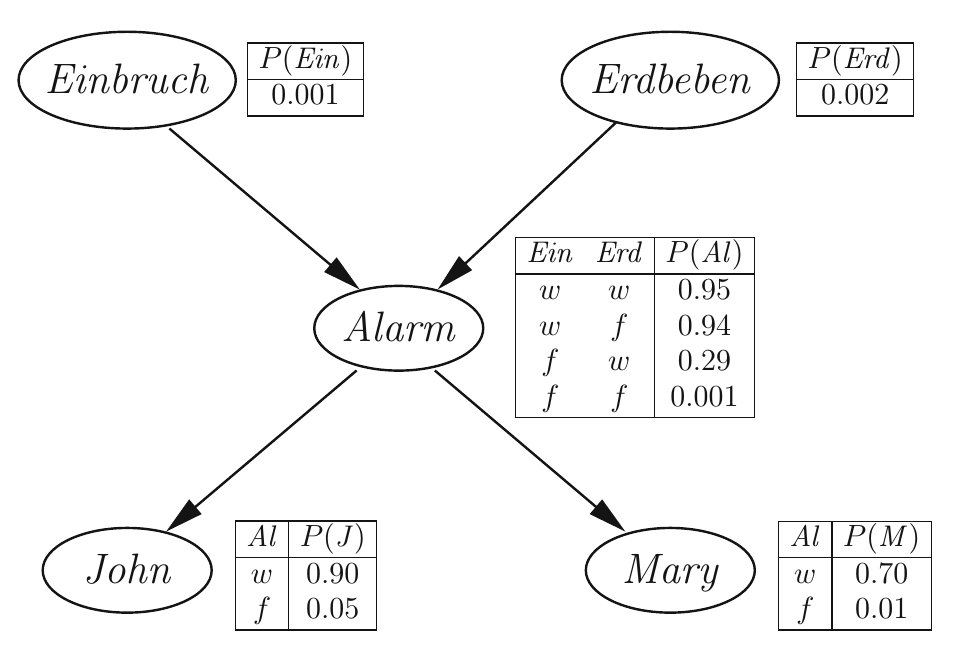
\includegraphics[scale=0.3]{bilder/bspNetz} 
\caption{Bayes'sches Netz des Alarmanlagen-/Erdbebenbeisiels \cite{Ertel16}}
\label{Agenten}
\end{figure}


Um die oben genannten Sachverhalte anschaulicher zu gestalten, kann man sie mit Hilfe eines Graphen visualisieren, siehe Abbildung 3.1.  Graphen bestehen im Allgemeinen aus Knoten und Kanten. Bei Graphen von Bayes'schen Netzen repräsentieren Knoten Variablen und Kanten stehen für eine bedingte Wahrscheinlichkeit. So gibt die Kante von \textit{Einbruch} nach \textit{Alarm} die Wahrscheinlichkeit \textit{P(Al$\vert$ Ein)} und \textit{P(Al$\vert$ $\overline{Ein}$)} wieder. In der Grafik ist auch eine Wahrheitstabelle enthalten. Die Abkürzungen \textit{w} und \textit{f} stehen für wahr und falsch. Die Tatsache, dass keine Kante von \textit{Einbruch} nach \textit{Erdbeben} zeigt, dass die Variablen unabhängig sind. Um die anderen Kanten zu verstehen, schauen wir uns erst einmal allgemein die \textit{Bedingte Unabhängigkeit} an. 
\subsection{Bedingte Unabhängigkeit}  
Zwei Variablen \textit{A} und \textit{B} sind stochastisch bedingt abhängig, wenn gilt:
\[ P(A,B\vert C) = P(A\vert C) * P(B\vert C)\]
Da in unserem Beispiel John und Mary unabhängig auf einen Alarm reagieren, gilt für das Ereignis \textit{P(J,M$\vert$ Al)} folgendes:
\[ P(J,M\vert Al) = P(J\vert Al) * P(M\vert Al)\]
Es handelt sich hier also auch um bedingt unabhängige Ereignisse. Ist nun ein Wert $\neq$ 0 für \textit{Al} bekannt (in diesem Beispiel ist der Wert für \textit{Al} diskret, er kann also nur 0 oder 1 sein), so redet man von einer Unabhängigkeit. Die Variablen \textit{J} hingegen sind nur bedingt unabhängig und nicht unabhängig. 
Für die Variablen \textit{J} und \textit{Ein} gilt folgendes:
\[ P(J,Ein\vert Al) = P(J\vert Al) * P(Ein\vert Al)\]
Die Erkenntnis aus der obigen Gleichung lautet: \textit{J} und \textit{Ein} sind unabhängig, gegeben \textit{Al}. Ebenso unabhängig sind auch \textit{J} und \textit{Erd} gegeben \textit{Al}, \textit{J} und \textit{Erd} gegeben \textit{Al}, \textit{M}, \textit{M} und \textit{Ein} gegeben \textit{Al} sowie \textit{M} und \textit{Erd} gegeben \textit{Al}. 

Mit dem Hintergrundwissen kann man nun konkrete Wahrscheinlichkeiten berechnen:
\[ P(J\vert Ein) = \frac{P(J\vert Ein)}{P(Ein)}  = \frac{P(J,Ein,Al) + P(J,Ein, \overline{Al}))}{P(Ein)} \]
Sprich: Die Wahrscheinlichkeit eines Anrufes von John wenn eingebrochen wurde.
Wir müssen hierfür noch \textit{P(J,Ein,Al)} bzw. \textit{P(J,Ein,Al)} kennen:
\[ P(J, Ein, Al) = P(J\vert Ein, Al) * P(Al\vert Ein) * P(Ein) = P(J\vert Al) * P(Al\vert Ein) * P(Ein) \] 
Dies können wir nun in die obere Gleichung einsetzen:
\[ P(J\vert EIn) =  \frac{P(J\vert	Al) * P(Al\vert Ein) * P(Ein) + P(J\vert \overline{Al}) * P(\overline{Al} \vert Ein) * P(Ein) }{P(Ein)}  \]
Durch Konditionieren erhält man:
\[ P(J\vert Al) * P(Al\vert Ein) + P(J\vert \overline{Al}) * P(\overline{Al} \vert Ein) \]
\textit{P(Al $\vert$ Ein)} und \textit{P($\overline{Al}$ $\vert$ Ein)} sind ohne weiteres noch nicht zu berechnen, also stellen wir hier einen Zusammenhang her:
\[ P(Al\vert Ein) = \frac{P(Al, Ein)}{P(Ein)} = \frac{P(Al,Ein,Erd) + P()Al,Ein, \overline{Erd} }{P(Ein)}  \]
\[ = \frac{P(Al\vert Ein, Erd) * P(Ein) * P(Erd) + P(Al\vert Ein, \overline{Erd}) * P(Ein) * P(\overline{Erd}) }{P(Ein)}\]
\[ = P(Al\vert Ein, Erd) * P(Erd) + P(Al\vert Ein, \overline{Erd}) * P(\overline{Erd}) \]
\[ = 0,95 * 0,002 + 0,94 * 0,998 = 0,94 \]
\[ P(\overline{Al}\vert Ein) = 1-0,94 = 0,06 \]
Diese zwei Zahlenwerte können wir nun in die Formel für \textit{P(J$\vert$ Ein)} einsetzen und erhalten:
\[ P(J\vert Ein) = 0,9 * 0,94 + 0,05 * 0,06 = 0,849 \]
Nun könne wir sagen, dass John mit einer Wahrscheinlichkeit von 84,9\% bei Einbrüchen anruft. Anhand des vorhandenen Bayes'schen Netzes kann man nun Wahrscheinlichkeiten für weitere Ereignisse berechnen. 
Die Anzahl der Einträge der zugehörigen Wahrheitstabelle beträgt nun nur noch \textit{n * (m-1) * $m^k$}, wobei \textit{k} die Anzahl der Elternknoten ist. Nach \cite{Ertel16}

